% $Header: /u/gcmpack/manual/s_under_dvlp/text/time_stepping_dvlp.tex,v 1.2 2010/08/24 22:46:34 jmc Exp $
% $Name:  $

\section{Other Time-stepping Options}
%\begin{rawhtml}
%<!-- CMIREDIR:dvlp-time-stepping: -->
%\end{rawhtml}

\subsection{Adams-Bashforth III}

\begin{figure}[ht]
\begin{center}
\resizebox{10cm}{!}{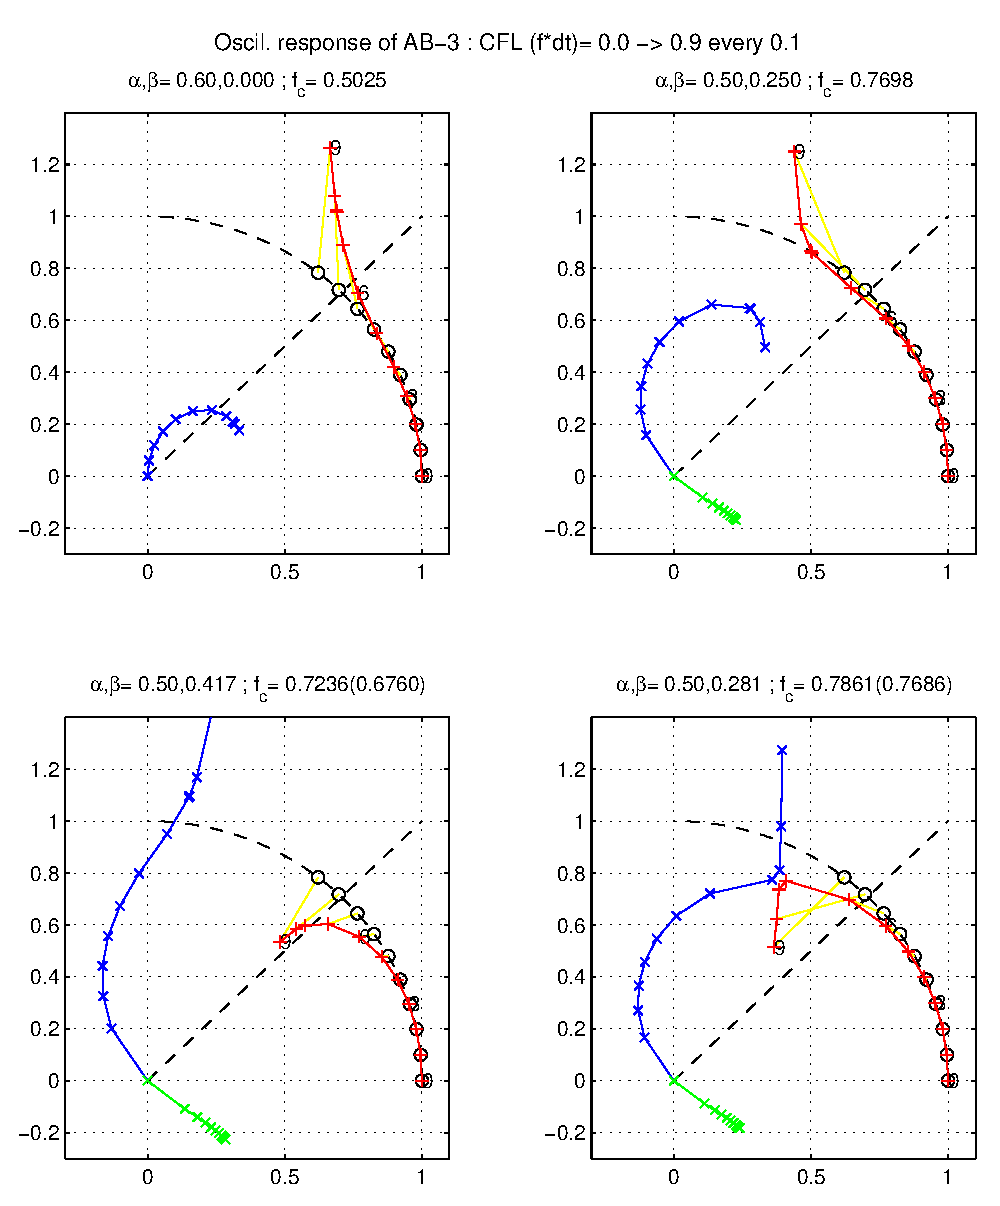
\includegraphics{under_dvlp/stab_AB3_oscil.eps}}
\end{center}
\caption{
Comparison of the oscillatory response of Adams-Bashforth scheme.
}
\label{fig:ab_oscill_response}
\end{figure}

As seen on fig.\ref{fig:adams-bashforth-respons}
The third-order Adams-Bashforth time stepping (AB-3) can be used instead 
of the default quasi-second order Adams-Bashforth (AB-2), 
with several advantages (see, e.g., \cite{durr:91}):
\begin{itemize}
\item higher accuracy.
\item stable with a longer time-step (for an oscillatory problem
like advection or Coriolis, stable up to a CFL of 0.72, 
compared to only 0.50 with AB-2 and $\epsilon_{AB} = 0.1$)
(fig.\ref{fig:ab_oscill_response})
\item no additional computation, but only requires to store one additional 
 time level.
\end{itemize}

The extrapolation forward in time of the tendency (replacing equation 
\ref{eq:adams-bashforth2} can be written:
\begin{equation}
G_\tau^{(n+1/2)} = ( 1 + \alpha_{AB} + \beta_{AB}) G_\tau^n
- ( \alpha_{AB} + 2 \beta_{AB}) G_\tau^{n-1}
+ \beta_{AB} G_\tau^{n-2}
\label{eq:adams-bashforth3}
\end{equation}
with $(\alpha_{AB},\beta_{AB}) = (1/2, 5/12)$ corresponding to the 
3rd order AB. One can also recover 
The quasi-2nd order AB corresponds to the particular case
$(\alpha_{AB},\beta_{AB}) = (1/2+\epsilon_{AB}, 0)$.

One can also extend the stability limit
up to a CFL of 0.786 for an oscillatory problem 
(see fig.\ref{fig:ab_oscill_response})
using $(\alpha_{AB},\beta_{AB}) = (0.5, 0.2811)$
but then the scheme is only 2nd order accurate.

\begin{figure}[ht]
\begin{center}
\resizebox{10cm}{!}{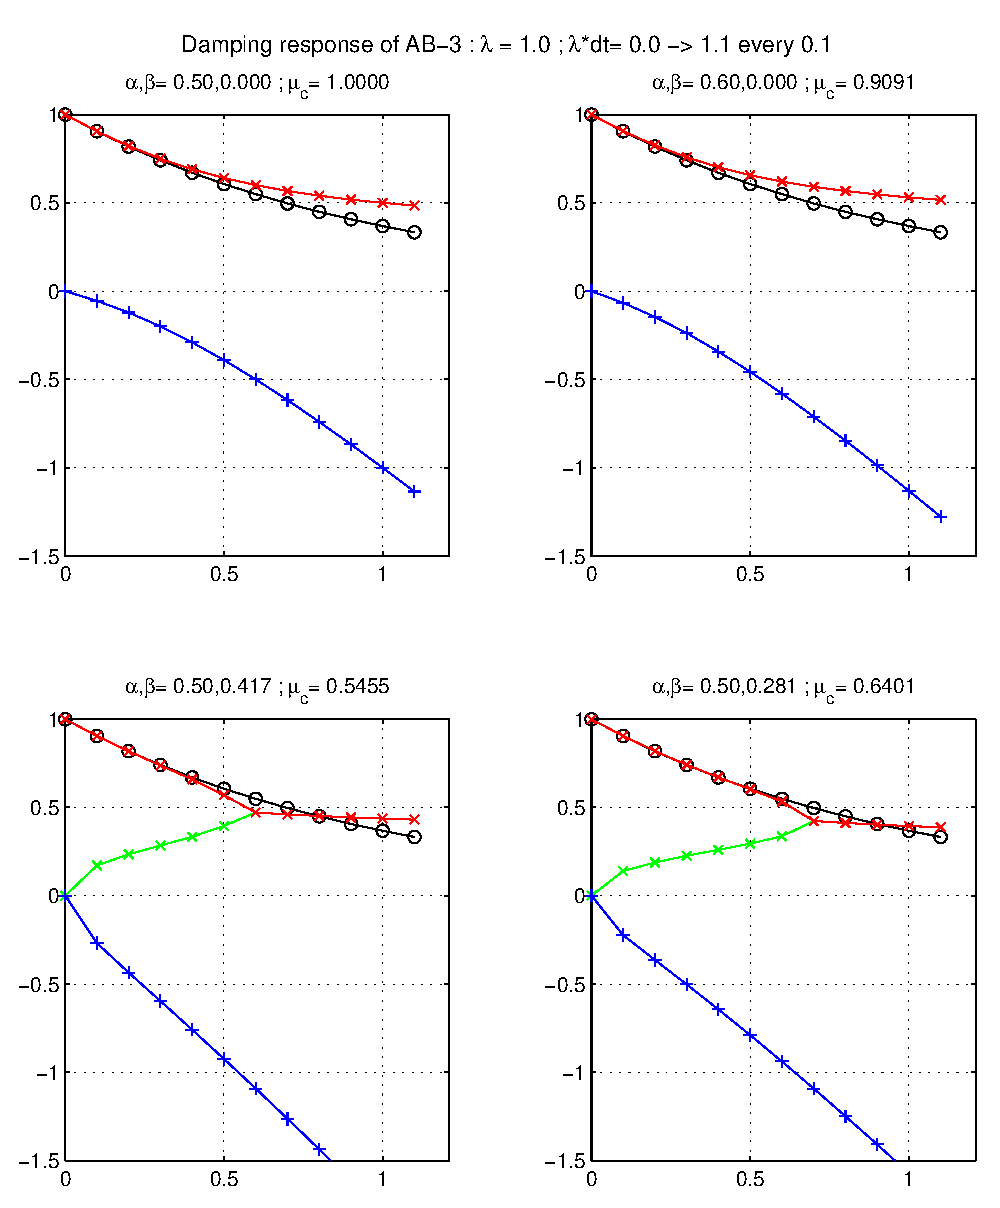
\includegraphics{under_dvlp/stab_AB3_dampR.eps}}
\end{center}
\caption{
Comparison of the damping (diffusion like) response of Adams-Bashforth schemes.
}
\label{fig:ab_damp_response}
\end{figure}

However, the behavior of the AB-3 for a damping problem (like diffusion)
is less favorable, since the stability limit is reduced to 
0.54 only (and 0.64 with $\beta_{AB} = 0.2811$) compared to 1. (and 0.9 
with $\epsilon_{AB} = 0.1$) with the AB-2 (see fig.\ref{fig:ab_damp_response}).

A way to enable the use of a longer time step is
to keep the dissipation terms outside the AB extrapolation
(therefore using a simple forward time-stepping) (setting
momDissip\_In\_AB=.FALSE. in main parameter file "data",
namelist PARM03), and use AB-3 for advection and Coriolis terms.

The AB-3 time stepping is activated by defining the option
\#define ALLOW\_ADAMSBASHFORTH\_3
in CPP\_OPTIONS.h
The parameters $\alpha_{AB},\beta_{AB}$ can be set from the
main parameter file "data" (namelist "PARM03") and their 
default values correspond to the 3rd order Adams-Bashforth.
A simple example is provided in verification/advect\_xy/input.ab3\_c4.

The AB-3 is not yet available for 
the vertical momentum equation (Non-Hydrostatic) and passive
tracers.

\subsection{Time-extrapolation of tracer (rather than tendency)}
 (to be continued ...)
